% !TEX root = ../notes_template.tex
\chapter{Vectors}\label{chp:vectors}

% \minitoc

\section{$n$-Vectors}
A collection of an ordered list of $n$ numbers is called an $n$-vector. We will use bold lower case alphabets to represent such vectors, and we will represent these as a column of numbers, which is referred to as a \textit{column vector}. We will look at \textit{row vectors} at a later stage. Consider the following example:
\[ \mf{x} = \bmxc x_1 \\ x_2 \\ \vdots \\x_n \emx \]

The elements of the $n$-vector $x_1, x_2, \ldots, x_n$ are called the \textit{components} of the vector $\mf{x}$; $x_i$ is the $i^{th}$ component of the vector $\mf{x}$. If these components are all real numbers, the set of all such $n$-vectors is the set $\mb{R}^n$.

\noindent \textbf{Where do we come across such $n$-vectors?} In many places, such as in physics, engineering, economics, medicine, etc. Any application where we deal with multiple pieces of information that can be represented as a list of numbers can be represented as an $n$-vector. When we deal with systems with multiple inputs, multiple output, or multiple states, we can represent these as $n$-vectors. We talk about the state of a system in a later chapter.

\section{Visualizing $n$-vectors}
The $n$-vectors can be visualized as points in $n$-dimensional space. For example, A 1-vector or just single real number or a \textit{scalar} can be thought of as a point on the real line. The 1-vector $x = 2.45$ is shown in Figure~\ref{fig:1-vector} is the red point. But we will find it useful to visualize a 1-vector as an arrow starting at the origin and ending at the point on the real line. The arrow is shown in blue in Figure~\ref{fig:1-vector}. 

\begin{figure}[b]
    \centering
    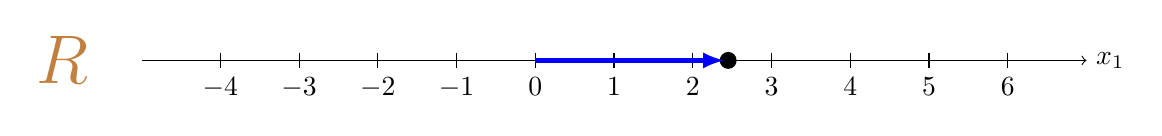
\begin{tikzpicture}
        \draw[->] (-5,0) -- (7,0) node[right] {$x_1$};
        \foreach \x in {,-4,-3,-2,0,-1,1,2,3,4,5,6}
            \draw (\x,0.1) -- (\x,-0.1) node[below] {$\x$};
        % Plot an example point and its corresponding arrow
        \draw[fill=black] (2.45,0) circle (0.1); % Smaller marker size
        \draw[-latex, ultra thick, blue] (0,0) -- (2.4,0); % Thicker arrow
        % Huge font for the label with brown color
        \node[font=\Huge, text=brown] at (-6, 0) {$\mathbb{R}$};
    \end{tikzpicture}
    \caption{The real line $\mb{R}$ contains the $1$-vectors.}
    \label{fig:1-vector}
\end{figure}

The elements of $\mb{R}^2$ are points on the plane, and we can visualize them as points in the plane. The 2-vectors $\mf{x} = \bmxc 2 \\ 3 \emx$ and $\mf{x} = \bmxc -3 \\ 1 \emx$ are shown in Figure~\ref{fig:2-vector}. A similar visualization is shown for $\mb{R}^3$ (Figure~\ref{fig:3-vector}), and for $\mb{R}^4$ and beyond you simply pretend that you can visualize things in your head like your instructor does.

\begin{figure}[t]
    \centering
    \begin{subfigure}[b]{0.45\textwidth}
        \centering
        \begin{tikzpicture}[scale=0.6]
            \draw[->, gray] (-5,0) -- (5,0) node[right] {$x_1$};
            \draw[->, gray] (0,-5) -- (0,5) node[above] {$x_2$};
            \foreach \x in {-4,-2,-1,2,4}
            \draw (\x,0.1) -- (\x,-0.1) node[below, gray] {$\x$};
            \foreach \y in {-4,-2,-1,2,4}
            \draw (0.1,\y) -- (-0.1,\y) node[left, gray] {$\y$};
            % Plot an example point and its corresponding arrow
            \draw[fill=black] (2,3) circle (0.1); % Marker for the point (2,3)
            \draw[-latex, ultra thick, blue] (0,0) --  (2,3) node[right, black] {$\mathbf{x} = \begin{bmatrix} 2 \\ 3 \end{bmatrix}$}; % Arrow with label
            
            \draw[fill=black] (-3,1) circle (0.1); % Marker for the point (-2,1)
            \draw[-latex, ultra thick, red] (0,0) --  (-3,1) node[left, black] {$\mathbf{y} = \begin{bmatrix} -3 \\ 1 \end{bmatrix}$}; % Arrow with label
            
            % Huge font for the label with brown color
            \node[font=\Huge, text=brown] at (-4, 4) {$\mathbb{R}^2$};
        \end{tikzpicture}
        \caption{The $\mathbb{R}^2$ plane contains the $2$-vectors.}
        \label{fig:2-vector}
    \end{subfigure}
    \begin{subfigure}[b]{0.45\textwidth}
        \centering
        \tdplotsetmaincoords{60}{120} % Set the view angle
        \begin{tikzpicture}[scale=0.7,tdplot_main_coords] % Set scale and use the main coordinates
            % Axis lines
            \draw[->, gray] (-5,0,0) -- (5,0,0) node[anchor=north east]{$x_1$};
            \draw[->, gray] (0,-5,0) -- (0,5,0) node[anchor=north west]{$x_2$};
            \draw[->, gray] (0,0,-5) -- (0,0,5) node[anchor=south]{$x_3$};
            \foreach \x in {-4,-2,,2,4}
                \draw (\x,0,0.1) -- (\x,0,-0.1) node[below, gray] {$\x$};
            \foreach \y in {-4,-2,,2,4}
                \draw (0.1,\y,0) -- (-0.1,\y,0) node[above right, gray] {$\y$};
            \foreach \z in {-4,-2,,2,4}
                \draw (0.1,0,\z) -- (-0.1,0,\z) node[above right, gray] {$\z$};
            % Points
            \draw[fill=blue] (1,2,3) circle (0.08);
            \draw[-latex, ultra thick, blue] (0,0,0) --  (1,2,3) node[above, black] {$\mathbf{x} = \bmx 1 \\ 2 \\ 1 \emx$}; 
            % Points
            \draw[fill=red] (2,-1,1) circle (0.08);
            \draw[-latex, ultra thick, red] (0,0,0) --  (2,-1,1) node[below left, black] {$\mathbf{y} = \bmx 2 \\ -1 \\ 1 \emx$}; 
             
            % Huge font for the label with brown color
            \node[font=\Huge, text=brown] at (2,-2,4.5) {$\mathbb{R}^3$};
        \end{tikzpicture}
        \caption{$\mb{R}^3$ contains the 3-vectors.}
        \label{fig:3-vector}
    \end{subfigure}
    \caption{The $\mb{R}^2$ and $\mb{R}^3$ sets.}
    \label{fig:combined}
\end{figure}

\section{Some Commonly Used $n$-vectors}
We will now define a some commonly used $n$-vectors that we will use in the course. 
\begin{itemize}
    \item \textbf{Zero vector:} The $n$-vector whose components are all zeros is called the \textit{zero vector}. $\mf{0} = \bmxc 0 \\ 0 \\ \vdots \\ 0\emx$
    \item \textbf{One vector:} The $n$-vector whose components are all ones is called the \textit{one vector}. $\mf{1} = \bmxc 1 \\ 1 \\ \vdots \\ 1\emx$
    \item \textbf{Unit vectors:} The $n$-vectors whose components are all zeros except for one component which is 1. These are called the \textit{standard basis vectors} and are denoted by $\mf{e}_1, \mf{e}_2, \ldots, \mf{e}_n$. The $n$-vector $\mf{e}_i$ has all components as zeros except for the $i^{th}$ component which is 1. For example, the unit vectors in $\mb{R}^2$ are:
    \[ \mf{e}_1 = \bmx 1 \\ 0\emx \quad \mf{e}_2 = \bmx 0 \\ 1 \emx  \]
\end{itemize}

\section{Operations on $n$-vectors}
There are many operations we can perform on $n$-vectors, but we will only focus on two operations for this:
\begin{itemize}
    \item \textbf{Scalar multiplication:} Given a scalar $c \in \mb{R}$ and an $n$-vector $\mf{x}$. The scalar multiplication operation produces another $n$-vector $c\mf{x}$ whose components are $cx_1, cx_2, \ldots, cx_n$. 
    \[ \mf{x} = \bmx 1 \\ 2\emx \longrightarrow 2 \mf{x} = \bmx  2\ct{1} \\ 2\ct{2} \emx = \bmx  2 \\ 8.2 \emx \]

    The geometric interpretation scalar multiplication is shown in Figure~\ref{fig:scalar-mult}. Scalar multiplication stretches or shrinks the vector without rotating it. When the scalar is positive the direction of the scaled vector is the same as the original vector, and when the scalar is negative the direction is opposite. When the scalar is zero, the scaled vector is the zero vector $\mf{0}$. 
    \begin{figure}[h!]
        \centering
        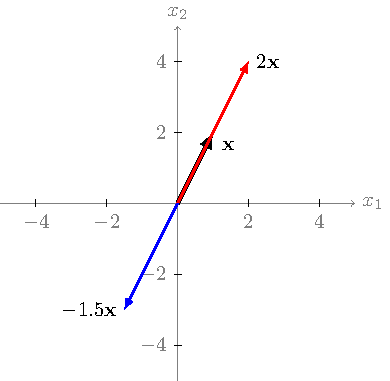
\includegraphics{figure/chapter01/vec-scale.pdf}
        \caption{Scalar multiplication of a vector.}
        \label{fig:scalar-mult}
    \end{figure}
    
    \item \textbf{Vector Addition:} Given two $n$-vectors $\mf{x}$ and $\mf{y}$, the vector addition operation, represented by $\mf{x} + \mf{y}$, producs another $n$-vector whose components are $x_1 + y_1, x_2 + y_2, \ldots, x_n + y_n$.
    \[ \mf{x} = \bmxc 1 \\ 3 \emx, \mf{y} = \bmxc 2 \\ 1 \emx \longrightarrow \mf{x} + \mf{y} = \bmxc 1 + 2 \\ 3 + 1 \emx = \bmxc 3 \\ 4 \emx \]
    
    \begin{figure}[h!]
        \centering
        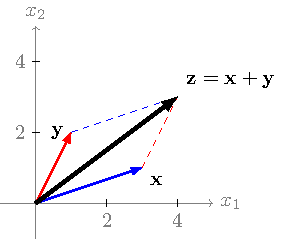
\includegraphics{figure/chapter01/vec-add-fig.pdf}
        \caption{Vector addition.}
        \label{fig:vec-add}
    \end{figure}

    The geometric interpretation the vector addition operation is shown in Figure~\ref{fig:vec-add}. Geometrically, the vector addition operation follows the parallelogram law of addition, where the resulting vector $\mf{x} + \mf{y}$ is a diagonal of the parallelogram formed by the two vectors $\mf{x}$ and $\mf{y}$. Another way to think about this, is that you first move along $\mf{x}$ to its end point, and starting from there then move along $\mf{y}$ to its end point or vice versa.

    You can add more than two vectors to obtain a new vector, like below:
    \[ \mf{w} = \mf{x} + \mf{y} + \mf{z} \]
    Geometrically, we can first apply the parallelogram law to $\mf{x}$ and $\mf{y}$, and then apply the parallelogram law to $\mf{x} + \mf{y}$ and $\mf{z}$ to get $\mf{w}$.
\end{itemize}


\section{Vector spaces}
Vector spaces are \textit{sets} with some special properites. More specifically, a vector space is a set $V$ of elements called \textit{vectors} that are closed under two operations called \textit{addition} and \textit{scalar multiplication}. This simply means that if you perfom these operations using elements from the set $V$, the result is also an element of the set $V$. A vector space must satisfy the following properties:
\begin{itemize}
    \item \textbf{Closure under addition:} For any two vectors $\mf{x}, \mf{y} \in V$, the sum $\mf{x} + \mf{y} \in V$.
    \item \textbf{Closure under scalar multiplication:} For any scalar $c \in \mb{R}$ and any vector $\mf{x} \in V$, the product $c\mf{x} \in V$.
    \item \textbf{Additive identity:} There exists a vector $\mf{0} \in V$ such that for any vector $\mf{x} \in V$, $\mf{x} + \mf{0} = \mf{x}$.
    \item \textbf{Additive inverse:} For any vector $\mf{x} \in V$, there exists a vector $-\mf{x} \in V$ such that $\mf{x} + (-\mf{x}) = \mf{0}$.
    \item \textbf{Commutativity of addition:} For any two vectors $\mf{x}, \mf{y} \in V$, $\mf{x} + \mf{y} = \mf{y} + \mf{x}$.
    \item \textbf{Associativity of addition:} For any three vectors $\mf{x}, \mf{y}, \mf{z} \in V$, $(\mf{x} + \mf{y}) + \mf{z} = \mf{x} + (\mf{y} + \mf{z})$.
    \item \textbf{Distributive property:} For any scalar $c \in \mb{R}$ and any two vectors $\mf{x}, \mf{y} \in V$, $c(\mf{x} + \mf{y}) = c\mf{x} + c\mf{y}$.
    \item \textbf{Distributive property:} For any two scalars $c, d \in \mb{R}$ and any vector $\mf{x} \in V$, $(c + d)\mf{x} = c\mf{x} + d\mf{x}$.
    \item \textbf{Associativity of scalar multiplication:} For any two scalars $c, d \in \mb{R}$ and any vector $\mf{x} \in V$, $(cd)\mf{x} = c(d\mf{x})$.
    \item \textbf{Multiplicative identity:} For any vector $\mf{x} \in V$, $1\mf{x} = \mf{x}$.
\end{itemize}
These properties are satisfied by the set $\mb{R}^n$ of $n$-vectors, and hence $\mb{R}^n$ is a vector space. Geometrically, the concept of a vector space corresponds to flat spaces that contain the origin. This will become more clear when we talk about subspaces. Notice that definition of the vector space given above does not make any specific mention of $n$-vectors. The definition is general and can be applied to any set of elements that satisfy the properties listed above. The following are some examples of vector spaces with the addition and scalar multiplication operations defined on them.

\begin{example}
    \textbf{Set of $m \times n$ matrices.} The set $M$ of all $m \times n$ matrices of real numbers is a vector space.
    \[ \mf{A} = \bmxc
        a_{11} & a_{12} & \cdots & a_{1n} \\
        a_{11} & a_{12} & \cdots & a_{1n} \\
        \vdots & \vdots & \ddots & \vdots \\
        a_{11} & a_{12} & \cdots & a_{1n}
    \emx, \,\, a_{ij} \in \mb{R} \]

    We define scalar multiplication and addition of matrices as follows:
    \[ c\mf{A} = \bmxc
        ca_{11} & ca_{12} & \cdots & ca_{1n} \\
        ca_{11} & ca_{12} & \cdots & ca_{1n} \\
        \vdots & \vdots & \ddots & \vdots \\
        ca_{11} & ca_{12} & \cdots & ca_{1n}
    \emx, \,\, c \in \mb{R} \]
    \[ \mf{A} + \mf{B} = \bmxc
        a_{11} + b_{11} & a_{12} + b_{12} & \cdots & a_{1n} + b_{1n} \\
        a_{11} + b_{11} & a_{12} + b_{12} & \cdots & a_{1n} + b_{1n} \\
        \vdots & \vdots & \ddots & \vdots \\
        a_{11} + b_{11} & a_{12} + b_{12} & \cdots & a_{1n} + b_{1n}
    \emx, \,\, \mf{A}, \mf{B} \in M
    \]
    Since each element of $c\mf{A}$ and $\mf{A} + \mf{B}$ is a real number, $M$ is a vector space.
    \label{example:matrix-vector-space}
\end{example}

\begin{example}
    \textbf{Set of polynomials of order $\leq n$.} Now we look at strange example of a vector space. The set $P_n$ of all polynomials of degree at most $n$ with real coefficients, defined over an interval $[a, b]$.
    \[ p\lp x \rp = \sum_{k=0}^{n-1} a_k x^k, \,\, x \in [a, b], \, a_k \in \mb{R} \]
    The set $P_n$ contains all polynomials of the form shown above. We define scalar multiplication and addition of polynomials as follows:
    \[ c p\lp x \rp = c \sum_{k=0}^{n-1} a_k x^k = \sum_{k=0}^{n-1} ca_k x^k, \,\, p\lp x\rp \in P \]
    \[ p\lp x \rp + q\lp x \rp = \sum_{k=0}^{n-1} a_k x^k + \sum_{k=0}^{n-1} b_k x^k = \sum_{k=0}^{n-1} \lp a_k + b_k \rp x^k, \,\, p\lp x \rp, q\lp x \rp \in P_n \]
    The set $P_n$ is a vector space because the sum and product of any two polynomials from $P_n$ is also a polynomial of degree at most $n$ with real coefficients.
    \label{example:polynomial-vector-space}
\end{example}

\begin{example}
    \textbf{Set of continuous functions.} The set $C\left[0, 1\right]$ of all continuous functions $f\lp x\rp$ over the time interval $x \in \left[ 0, 1\right]$ is a vector space. We define scalar multiplication and addition of functions as follows:
    \[ c f\lp x \rp = c f\lp x \rp, \,\, f\lp x \rp \in C\lp 0, 1 \rp \]
    \[ f\lp x \rp + g\lp x \rp = f\lp x \rp + g\lp x \rp, \,\, f\lp x \rp, g\lp x \rp \in C\lp 0, 1 \rp \]
    The set $C\lp 0, 1 \rp$ is a vector space because the sum and product of any two continuous functions from $C\lp 0, 1 \rp$ is also a continuous function.
    \label{example:continuous-function-vector-space}
\end{example}

\section{Subspaces -- ``Little'' Vector Spaces}
These are little subspaces in the sense that they are subsets of a larger vector space that are themselves vector spaces. More formally, a subspace $U$ of a vector space $V$ is a subset of $V$ that is itself a vector space. The subspace $U$ of the vector space $V$ must satisfy the following properties:
\begin{itemize}
    \item \textbf{Closure under addition:} For any two vectors $\mf{x}, \mf{y} \in U$, the sum $\mf{x} + \mf{y} \in U$.
    \item \textbf{Closure under scalar multiplication:} For any scalar $c \in \mb{R}$ and any vector $\mf{x} \in U$, the product $c\mf{x} \in U$.
\end{itemize}
One immediate consequence of the above definition is that hte zero element of the vector space $V$ must be present in every subspace of $V$. If the zero element is not in a subset, then it cannot be a subspace. Geometrically subspace are flat structures (or surfaces or manifolds) in $\mb{R}^n$ (or the parent vector space) that contain the origin, and extends infinitely. Let's look at some examples of subspaces of $\mb{R}^2$ and $\mb{R}^3$, which are easier to visualize.

\begin{example}
    \textbf{A straight line through the origin.} We know that $\mb{R}^2$ is a vector space. Now consider the set of all points in $\mb{R}^2$ that lie on a straight line passing through the origin, defined as follows:
    \[ S = \lc \mf{x} \, : \, x = \bmx x_1 \\ x_2 \emx \in \mb{R}^2, \, x_1 = m \cdot x_2, \, m \in \mb{R} \rc \]
    How do we verfiy this is a subspace of $\mb{R}^2$? The definition above shows that any $x$ in $S$ comes from $\mb{R}^2$, which means its a subset of $\mb{R}^2$. Figure~\ref{fig:subspace1} shows the set $S$ for $m = 2$.
    \begin{figure}[h]
    \centering
    \begin{subfigure}[b]{0.32\textwidth}
        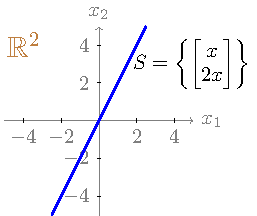
\includegraphics{figure/chapter01/subspace1(a).pdf}
        \caption{A subspace of $\mb{R}^2$.}
        \label{fig:subspace1}
    \end{subfigure}
    \begin{subfigure}[b]{0.32\textwidth}
        \centering
        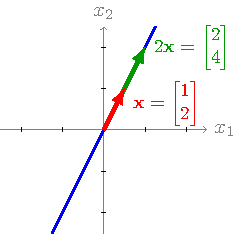
\includegraphics{figure/chapter01/subspace1(b).pdf}
        \caption{Vector scaling.}
        \label{fig:subspace1-scale}
    \end{subfigure}
    \begin{subfigure}[b]{0.32\textwidth}
        \centering
        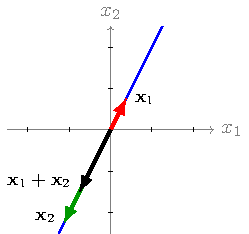
\includegraphics{figure/chapter01/subspace1(c).pdf}
        \caption{Vector addition.}
        \label{fig:subspace1-addition}
    \end{subfigure}
    \caption{Example of a subspace of $\mb{R}$. (a) Shows the set of all points in $\mb{R}^2$ corresponding to the subset $S = \left\{ \bmxc x \\ 2 x\emx\right\} \subset \mb{R}^2$. (b) Shows that the set $S$ is closed under scalar multiplication. Take any vecotr from the line, and scale it and it remains on that blue line. (c) Shows that $S$ is closed under vector addition. If we take any two vectors from the blue line and add them, the resulting vector remains in the blue line.}
    \end{figure}    
    
    \noindent How do we verify if $S$ is a subspace of $\mb{R}^2$? We need to now verify that $S$ satisfies the properties of a vector space.
    \begin{enumerate}
        \item First, let's check if $S$ contains the zero vector. If it does not contain the zero vector, then it cannot be a subspace. The elements from $S$ are of the form $\bmxc x \\ m x\emx$, thus if we choose $x = 0$, then we get $\bmx 0 \\ 0 \emx \in S$. So, $S$ contains the zero vector. This means that $S$ can be a subspace space of $\mb{R}^2$.
        \item Let's verify vector scaling. Scaling the element $\bmxc x \\ m x \emx \in S$ by a scalar $c$ we get,
        \[ c \bmxc x \\ m x\emx = \bmxc c x \\ c m x \emx = \bmxc c x \\ m \pp{c x} \emx = \bmxc y \\ m y\emx, \quad \text{where} \,\, y = c x \in \mb{R} \]
        This means that $c\bmxc x \\ m x\emx$ belongs to $S$, this the set $S$ is closed under scalar multiplication. This still means that $S$ can be a subspace of $\mb{R}^2$.
        \item Let's verify vector addition. Adding two elements $\bmxc x_1 \\ m x_1\emx, \bmxc x_2 \\ m x_2\emx \in S$ we get,
        \[ \bmxc x_1 \\ m x_1\emx + \bmxc x_2 \\ m x_2\emx = \bmxc x_1 + x_2 \\ m x_1 + m x_2 \emx = \bmxc y_1 \\ m y_1\emx, \quad \text{where} \,\, y_1 = x_1 + x_2 \in \mb{R} \]
        This means that $\bmxc y_1 \\ m y_1\emx$ belongs to $S$, this the set $S$ is closed under vector addition. This means that $S$ is a subspace of $\mb{R}^2$.
    \end{enumerate}
    Since, the subset $S$ is closed under both vector addition and scalar multiplication, it is a subspace of $\mb{R}^2$.
    \label{example:subspace-straight-line}
\end{example}

\begin{example}
    \textbf{A straight line not through the origin.} Consider the set of all points in $\mb{R}^2$ of the following form:
    \[ S = \lc \mf{x} \, : \, x = \bmxc x \\ m x + c \emx \in \mb{R}^2, \, m, c \in \mb{R} \rc \]
    This is shown in the Figure~\ref{fig:nosubspace1}.

    How do we verfiy this is a subspace of $\mb{R}^2$? The definition above shows that any $x$ in $S$ comes from $\mb{R}^2$, which means its a subset of $\mb{R}^2$. Figure~\ref{fig:nosubspace1} shows the set $S$ for $m = -\frac{1}{2}$ and $c = 1$.
    \noindent How do we verify if $S$ is a subspace of $\mb{R}^2$? We need to now verify that $S$ satisfies the properties of a vector space.
    \begin{enumerate}
        \item First, let's check if $S$ contains the zero vector. If it does not contain the zero vector, then it cannot be a subspace. The elements from $S$ are of the form $\bmxc x \\ m x + c\emx$, thus if we choose $x = 0$, then we get $\bmx 0 \\ c \emx \in S$. So, $S$ does not contain the zero vector, which implies that $S$ is not a subspace space of $\mb{R}^2$. We need not check the other two conditions; but we will test them just to see which of these two fails.
        \item Scaling the element $\bmxc x \\ m x + c \emx \in S$ by a scalar $d$ we get,
        \[ d \bmxc x \\ m x + c\emx = \bmxc d x \\ d m x + d c \emx = \bmxc d x \\ m \pp{d x} + dc \emx \neq \bmxc y \\ m y + c\emx, \quad \text{where} \,\, y = d x \in \mb{R} \]
        This means that $d \bmxc x \\ m x + c\emx \notin S$. Thus, the set $S$ is closed under scalar multiplication. Another confirmation that it is not a subspace. This can be seen in Figure~\ref{fig:nosubspace1-scale}, which shows that when we choose an elment from $\mf{x}$ (red arrow) from $S$ (blue line), the scaled version of this vector leaves the set $S$, i.e., the tip of the green arrow does not stay on the blue line.
        \item Let's verify vector addition. Adding two elements $\bmxc x_1 \\ m x_1 + c\emx, \bmxc x_2 \\ m x_2 + c\emx \in S$ we get,
        \[ \bmxc x_1 \\ m x_1 + c\emx + \bmxc x_2 \\ m x_2 + c\emx = \bmxc x_1 + x_2 \\ m x_1 + m x_2 + 2c \emx \neq \bmxc y_1 \\ m y_1 + c\emx, \quad \text{where} \,\, y_1 = x_1 + x_2 \in \mb{R} \]
        This means that $\bmxc x_1 \\ m x_1 + c\emx + \bmxc x_2 \\ m x_2 + c\emx \notin S$. Thus the set $S$ is closed under vector addition. We see this geometrically in Figure~\ref{sub@fig:nosubspace1-addition}, where the sum of two vectors in $S$ does not stay in the set $S$. Even though the tips of the green and red arrow are on the blue line, the tip of the black arrow is not on the blue line.
    \end{enumerate}
    Since, the subset $S$ is closed under both vector addition and scalar multiplication, it is a subspace of $\mb{R}^2$.
    \begin{figure}[h]
        \centering
        \begin{subfigure}[b]{0.32\textwidth}
            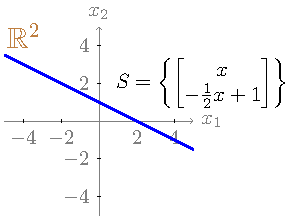
\includegraphics{figure/chapter01/nosubspace1(a).pdf}
            \caption{Not a subspace of $\mb{R}^2$.}
            \label{fig:nosubspace1}
        \end{subfigure}
        \begin{subfigure}[b]{0.32\textwidth}
            \centering
            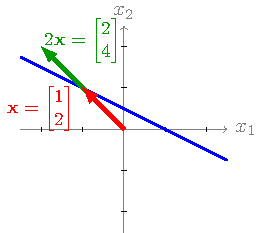
\includegraphics{figure/chapter01/nosubspace1(b).pdf}
            \caption{Vector scaling.}
            \label{fig:nosubspace1-scale}
        \end{subfigure}
        \begin{subfigure}[b]{0.32\textwidth}
            \centering
            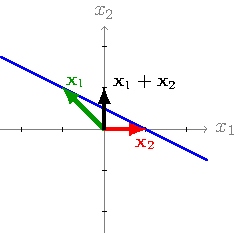
\includegraphics{figure/chapter01/nosubspace1(c).pdf}
            \caption{Vector addition.}
            \label{fig:nosubspace1-addition}
        \end{subfigure}
        \caption{Example of a subspace of $\mb{R}$. (a) Shows the set of all points in $\mb{R}^2$ corresponding to the subset $S = \left\{ \bmxc x \\ 2 x\emx\right\} \subset \mb{R}^2$. (b) Shows that the set $S$ is closed under scalar multiplication. Take any vecotr from the line, and scale it and it remains on that blue line. (c) Shows that $S$ is closed under vector addition. If we take any two vectors from the blue line and add them, the resulting vector remains in the blue line.}
    \end{figure}
    \label{example:nosubspace-straight-line}
\end{example}

\begin{example}
    \textbf{A parabola through the origin.} Consider the set of all points in $\mb{R}^2$ of the following form:
    \[ S = \lc \mf{x} \, : \, x = \bmxc x \\ \frac{1}{2}x^2 \emx \in \mb{R}^2, \, m, c \in \mb{R} \rc \]

    This is not a subspace of $\mb{R}^2$. This is geometrically depicted in Figure~\ref{fig:nosubspace2}, Figure~\ref{fig:nosubspace2-scale} and Figure~\ref{fig:nosubspace2-addition}. You are encouraged to verify this algebraically by checking the properties of a vector space.

    \begin{figure}[h]
        \centering
        \begin{subfigure}[b]{0.32\textwidth}
            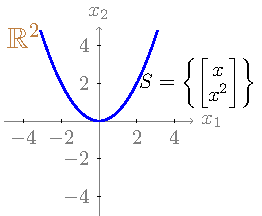
\includegraphics{figure/chapter01/nosubspace2(a).pdf}
            \caption{Not a subspace of $\mb{R}^2$.}
            \label{fig:nosubspace2}
        \end{subfigure}
        \begin{subfigure}[b]{0.32\textwidth}
            \centering
            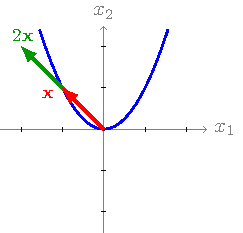
\includegraphics{figure/chapter01/nosubspace2(b).pdf}
            \caption{Vector scaling.}
            \label{fig:nosubspace2-scale}
        \end{subfigure}
        \begin{subfigure}[b]{0.32\textwidth}
            \centering
            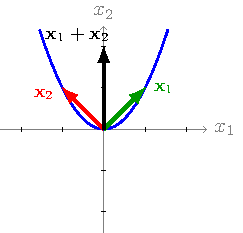
\includegraphics{figure/chapter01/nosubspace2(c).pdf}
            \caption{Vector addition.}
            \label{fig:nosubspace2-addition}
        \end{subfigure}
        \caption{Example of a subspace of $\mb{R}$. (a) Shows the set of all points in $\mb{R}^2$ corresponding to the subset $S = \left\{ \bmxc x \\ 2 x\emx\right\} \subset \mb{R}^2$. (b) Shows that the set $S$ is closed under scalar multiplication. Take any vecotr from the line, and scale it and it remains on that blue line. (c) Shows that $S$ is closed under vector addition. If we take any two vectors from the blue line and add them, the resulting vector remains in the blue line.}
    \end{figure}
    \label{example:nosubspace-parabola}
\end{example}

\section{Linear combinations and others}
Linear combination is an \textit{algebraic operation} performed on a set of vectors. We can combine the two fundamental operations on vectors into a single operation called the \textit{linear combination} of a set of vectors. Given a set of vectors $\mf{v}_1, \mf{v}_2, \ldots, \mf{v}_m \in \mb{R}^n$ and scalars $c_1, c_2, \ldots, c_n \in \mb{R}$, the linear combination of the vectors is given by:
\begin{equation}
    \mf{v} = c_1 \mf{v}_1 + c_2 \mf{v}_2 + \cdots + c_n \mf{v}_m \in \mb{R}^n
    \label{eq:linear-comb}
\end{equation}
Notice that the linear cominations of single vector $\mf{v}_1$ are simply different scaled versions of the vector $c_1 \mf{v}_1$. Linear cominations are the bread-and-butter of linear algebra and we will encounter them again and again. An informal way to think of a linear combination of a set of vectors as process of mixing the set of vectors together with the corresponding scalar $c_i$ determining the amount of a vector in the mixture. There are other types of combinations of vectors, which we will not discuss further in this book.
\begin{itemize}
    \item \textbf{Affine combination:} $\mf{v} = c_1 \mf{v}_1 + c_2 \mf{v}_2 + \cdots + c_n \mf{v}_m, \quad \sum_{i=1}^{m} c_i = 1$
    \item \textbf{Convex combinations:} $\mf{v} = c_1 \mf{v}_1 + c_2 \mf{v}_2 + \cdots + c_n \mf{v}_m, \quad c_i \geq 0, \,\, \sum_{i=1}^{m} c_i = 1$
    \item \textbf{Conic combinations:} $\mf{v} = c_1 \mf{v}_1 + c_2 \mf{v}_2 + \cdots + c_n \mf{v}_m, \quad c_i \geq 0$
\end{itemize}

\section{Linear independece of a set of vectors}
Linear independece is a \textit{property} of a set of vectors; a set of vector is either linearly independent or linearly dependent. The concept of linear independence is easy to understand the but the algebraic condition for independence can seem a bit unintuitive. A set of vectors is said to be \text{linearly independent} if no vector in the set can be expressed as a linear combination of the other vectors in the set. 

More formally, a set of vectors $V = \lc \mf{v}_i \rc_{i=1}^{m}$ is said to be linearly independent if and only if the only way to produce the zero vector $\mf{0}$ through the linear combination of the set $V$ is by setting all the scalars to zero, i.e.,
\begin{equation}
    c_1 \mf{v}_1 + c_2 \mf{v}_2 + \cdots + c_n \mf{v}_m = \mf{0} \quad \text{if and only if} \quad c_1 = c_2 = \cdots = c_m = 0
    \label{eq:linear-indep}
\end{equation}
To understand this better, let's assume that the set $V$ is linear dependent and let's assume that the vector $\mf{v}_m$ can be represented as the linear combination of the vectors $\mf{v}_1, \mf{v}-2, \cdots \mf{v}_{m-1}$. This means that there exist a set of scalar $\alpha_i, \,\, 1 \leq i \leq m-1$, such that
\[ \alpha_1 \mf{v}_1 + \alpha_2 \mf{v}_2 + \cdots + \alpha_{m-1}\mf{v}_{m-1} = \mf{v}_m \]
Multiplying both sides by a scalar $c_m \neq 0$ we get,
\[ \begin{split}
    c_m\alpha_1 \mf{v}_1 + c_m\alpha_2 \mf{v}_2 + \cdots + c_m\alpha_{m-1}\mf{v}_{m-1} &= c_m\mf{v}_m \\
    \implies c_m\alpha_1 \mf{v}_1 + c_m\alpha_2 \mf{v}_2 + \cdots + c_m\alpha_{m-1}\mf{v}_{m-1} - c_m\mf{v}_m &= \mf{0}
\end{split} \]
This implies that there exist a set of scalar $c_i = c_m\alpha_i, \,\, 1 \leq i \leq m-1$, and $c_m$ such that $c_1 \mf{v}_1 + c_2 \mf{v}_2 + \cdots + c_m \mf{v}_m = \mf{0}$, where not all $c_i$ are zero. So when a set is linearly dependent, then there are scalars $c_i$, not all zero, such that the linear combination of the vectors from $V$ with these scalars produces the zero vector.

Now, let's assume that the set $V$ is linearly independent, that is no vector in the set $V$ can be expressed as a linear combination of other vectors in that set. And let's assume that there are scalars $c_i$, not all zero, such that the linear combination of the vectors from $V$ with these scalars produces the zero vector, i.e.,
\[ \begin{split}
    c_1 \mf{v}_1 + c_2 \mf{v}_2 + \cdots + c_m \mf{v}_m &= \mf{0} \\
    \implies \frac{c_1}{c_m} \mf{v}_1 + \frac{c_2}{c_m} \mf{v}_2 + \cdots + \frac{c_{m-1}}{c_m}\mf{v}_{m-1} &= \mf{v}_m, \,\, c_m \neq 0
\end{split} \]
But this a contradiction because we have just expressed $\mf{v}_m$ is expressed as a linear combination of the vectors $\mf{v}_1, \mf{v}_2, \cdots \mf{v}_{m-1}$.

\section{Span of a set of vectors}
So, linear combinations of a set of vectors $V = \lc \mf{v}_i \rc_{i=1}^{m}$ ($\mf{v}_i \in \mb{R}^n$) is a way of generating new vectors not in that set. All we need to do is choose a random set of real numbers $\lc c_i \rc_{i=1}^{m}$, and ``mix'' the vectors $\mf{v}_i$ from the set using these as weights. Clearly there are infinite number of vectors we could generate through this process, and we can put them all together in a set. And this set has a name -- the \textit{span} of the set $V$. The span of a set of vectors $V = \lc \mf{v}_i \rc_{i=1}^{m}$ is denoted by $\text{span}\lp V \rp$ and is defined as:
\begin{equation}
    \text{span}\lp V \rp = \lc c_1 \mf{v}_1 + c_2 \mf{v}_2 + \cdots + c_n \mf{v}_m \, : \, c_i \in \mb{R} \rc \subseteq \mb{R}^n
    \label{eq:span-vec}
\end{equation}
Its clear that this will be a subset of $\mb{R}^n$, but it turns out it is also a subspace of $\mb{R}^n$. Why? Can you verify this fact algebraically? (\textit{Hint}: Just follow the steps in Examples~\ref{example:subspace-straight-line}-\ref{example:nosubspace-parabola}).

Geometrically, this means that the $\text{span}\pp{V}$ will be a flat surface in $\mb{R}^n$. Which means that the linear combination operation generates vectors that lie on a flat surface spanned by the vectors emmployed in the linear combination.

\begin{figure}[h]
    \centering
    \begin{subfigure}[b]{0.32\textwidth}
        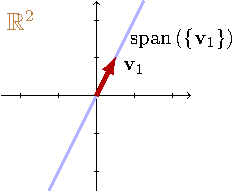
\includegraphics{figure/chapter01/span(a).pdf}
        \caption{Not a subspace of $\mb{R}^2$.}
        \label{fig:span1}
    \end{subfigure}
    \begin{subfigure}[b]{0.32\textwidth}
        \centering
        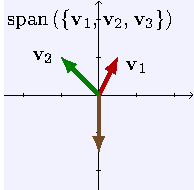
\includegraphics{figure/chapter01/span(b).pdf}
        \caption{Vector scaling.}
        \label{fig:span2}
    \end{subfigure}
    \begin{subfigure}[b]{0.32\textwidth}
        \centering
        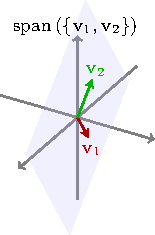
\includegraphics{figure/chapter01/span(c).pdf}
        \caption{Vector addition.}
        \label{fig:span3}
    \end{subfigure}
    \caption{Span of a set of vectors in $\mb{R}^2$ and $\mb{R}^3$.}
\end{figure}

\section{How big is a vector?}
The size of a vector is an extension of the idea of the magnitude of a real number. The magnitude of a real number $a \in \mb{R}$ tells us how big the number is irrespective of its sign:
\begin{equation}
    \vert a \vert = \begin{cases} a, & a \geq 0 \\ -a, & a < 0 \end{cases}
    \label{eq:magnitude-real}
\end{equation}

The ``magnitude'' or size of an element of a vector space (such as $\mb{R}^n$) is called the \textit{norm} of the vector. The norm of a vector is a function that maps a vector to a non-negative real number, and satisfies the following properties:
\begin{itemize}
    \item \textbf{Non-negativity:} For any vector $\mf{x} \in \mb{R}^n$, $\norm{\mf{x}} \geq 0$.
    \item \textbf{Definiteness:} The norm of a vector is zero if and only if the vector is the zero vector, i.e., $\norm{\mf{x}} = 0$ if and only if $\mf{x} = \mf{0}$.
    \item \textbf{Homogeneity:} Scaling a vector by a scalar $c$, scales the norm of the vector by $\vert c \vert$. For any vector $\mf{x} \in \mb{R}^n$ and any scalar $c \in \mb{R}$, $\norm{c\mf{x}} = \vert c \vert \norm{\mf{x}}$.
    \item \textbf{Triangle inequality:} For any vectors $\mf{x}, \mf{y} \in \mb{R}^n$, $\norm{\mf{x} + \mf{y}} \leq \norm{\mf{x}} + \norm{\mf{y}}$.
\end{itemize}
According to this definition, the magnitude of real numbers (Eq.~\ref{eq:magnitude-real}) is a norm of the vector $\mb{R}$. The most common norm of a vector is the \textit{Euclidean norm} or the \textit{2-norm} of a vector. The Euclidean norm of a vector $\mf{x} = \bmxc x_1 \\ x_2 \\ \vdots \\ x_n \emx$ is defined as:
\begin{equation}
    \norm{\mf{x}}_2 = \sqrt{x_1^2 + x_2^2 + \cdots + x_n^2}
    \label{eq:euclidean-norm}
\end{equation}
We are well-versed with this as the length of a vector in $\mb{R}^2$ and $\mb{R}^3$. The subscript $2$ in Eq.~\ref{eq:euclidean-norm} is used to indicate that it is the 2-norm, which is a special case of a general class of norms in $\mb{R}^n$ -- the \textit{p-norm}. The \textit{p-norm} is defined as the following:
\begin{equation}
    \norm{\mf{x}}_p = \lp \sum_{i=1}^{n} \vert x_i \vert^p \rp^{1/p}, \,\, p \in \mb{Z}, \,\, p \geq 1
    \label{eq:p-norm}
\end{equation}
Apart from the \textit{2-norm}, the \textit{1-norm} and the \textit{$\infty$-norm} are also commonly used norms, which are defined as the following:
\begin{equation}
    \norm{\mf{x}}_1 = \sum_{i=1}^{n} \vert x_i \vert, \quad \quad \quad \norm{\mf{x}}_{\infty} = \max_{i} \vert x_i \vert
    \label{eq:1-infinity-norm}
\end{equation}
The \textit{1-norm} is the sum of the absolute value of the elements of the vector, and the \textit{$\infty$-norm} is the maximum of the absolute value of the elements of the vector. The \textit{1-norm} is also called the \textit{Manhattan norm} or the \textit{Taxicab norm} because it measures the distance between two points in a city if you can only travel along the grid of streets.


\begin{boxedstuff}
    \begin{problem}
        Why does the $\infty$-norm measure have this weird looking definition compared to the other $p$-norms?
        \begin{solution}
            Consider the vector $\mf{x} \in \mb{R}^n$, and $x_{max} = \max_{0 \leq i \leq n} \vert x_i \vert$; let's also assume that the $j^{th}$ element of $\mf{x}$ has the maximum absolute value, i.e. $x_{max} = \vert x_j \vert$. The $p$-norm is defined as the following:
            \[ \begin{split} 
                \norm{\mf{x}}_p &= \lp \sum_{i=1}^{n} \vert x_i \vert^p \rp^{1/p} = x_{max} \lp 1 + \sum_{\substack{1 \leq i \leq n \\ i \neq j}} \lv \frac{x_i}{x_j} \rv^p \rp^{1/p} = x_{max}\lp N \rp^{1/p}\\
            \end{split}
            \]
            where, $N$ is a real number between $1$ and $n$, because $\vert \frac{x_i}{x_j} \vert \leq 1$ (why?). Now, if we increase the value of $p$ to infinity, then the term $\lim_{p \to infty} \lp N \rp^{1/p}= 1$. Thus, we have $\lV \mf{x} \rV_{\infty} = \lim_{p \to \infty} \lV \mf{x} \rV_p = x_{max} = \max_{i} \lv x_i \rv$.
        \end{solution}
    \end{problem}
\end{boxedstuff}

\subsection{Geometry of the p-norms}
In the case of real numbers, the set of all numbers with a magnitude of $1$ is the set $\lc -1, 1 \rc$. We can plot these points in the real line as below.

% Figure showing the loucs of all points with magnitude 1
% on the real line.
\begin{figure}[h]
    \centering
    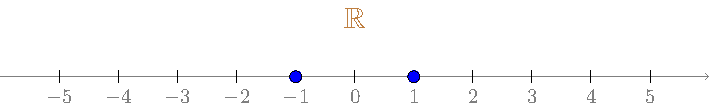
\includegraphics{figure/chapter01/mag-locus.pdf}
    \caption{The set of all real numbers with magnitude $1$. This set contains two numbers $\lc -1, 1 \rc$.}
    \label{fig:real-line-1-norm}
\end{figure}

In $\mb{R}^2$, the set of all vectors from $\mb{R}^2$ with a \textit{2-norm} of $1$ is the unit circle. The following figure shows the set of all points in $\mb{R}^2$ with unit 1, 2, $p$, and $\infty$ norm.

\begin{figure}[h]
    \centering
    \begin{subfigure}[b]{0.24\textwidth}
        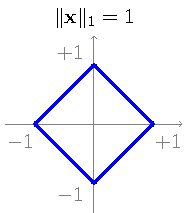
\includegraphics{figure/chapter01/norm1.pdf}
        \caption{1-norm}
        \label{fig:norm1}
    \end{subfigure}
    \begin{subfigure}[b]{0.24\textwidth}
        \centering
        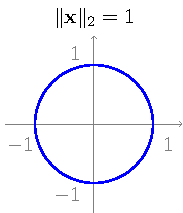
\includegraphics{figure/chapter01/norm2.pdf}
        \caption{2-norm}
        \label{fig:norm2}
    \end{subfigure}
    \begin{subfigure}[b]{0.24\textwidth}
        \centering
        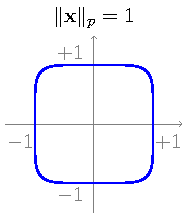
\includegraphics{figure/chapter01/normp.pdf}
        \caption{$p$-norm}
        \label{fig:normp}
    \end{subfigure}
    \begin{subfigure}[b]{0.24\textwidth}
        \centering
        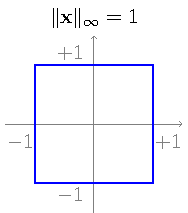
\includegraphics{figure/chapter01/norminf.pdf}
        \caption{$\infty$-norm}
        \label{fig:norminf}
    \end{subfigure}
    \caption{Locus of all points with unit 1, 2, $p$, and $\infty$ norms in $\mb{R}^2$.}
\end{figure}

\begin{boxedstuff}
    \begin{problem}
        Can you explain why the different norms have these shapes? 
    \end{problem}
    \begin{problem}
        Can you write a Python program to generate the above plots for different values of $p = 1, 2, 3, 10$ and $\infty$?
    \end{problem}
    \begin{problem}
        Can describe what these 1, 2, $p$ and $\infty$ norms will look like in $\mb{R}^3$?
    \end{problem}
\end{boxedstuff}

\section{How similar are two vectors?}
The idea of how similar two or more vectors are is an important topic  in data analysis, in particular in classification problems in machine learning. Vectors that are ``similar'' somehow belong to the same ``category'' or ``class'', while vectors that are ``dissimilar'' belong to different categories or classes. There are various ways to measure the similarity between two vectors. We will look at two methods in this section where similarity is mesasured by computing the distance between two vectors or by computing the angle between two vectors.

\subsection{Distance between two vectors}
\begin{wrapfigure}{r}{0.35\textwidth}
    \centering
    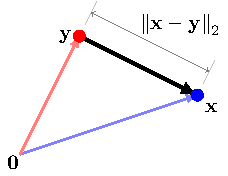
\includegraphics[width=0.95\linewidth]{figure/chapter01/dist-demo.pdf}
    \caption{Distance between two vectors.}
    \label{fig:distance1}
\end{wrapfigure}
The logic here is that similar vectors correspond to points that are close together, while disimilar vectors are father away. We can make use of the norm to compute the distance between two vectors $\mf{x}, \mf{y} \in \mb{R}^n$. Since the the difference between these two vectors $\mf{x} - \mf{y}$ is also another vector, we can compute the distance between vectors $\mf{x}$ and $\mf{y}$ as the norm of the vector $\mf{x} - \mf{y}$ (Figure~\ref{fig:distance1}).
\[ \text{Distance between } \mf{x} \text{ and } \mf{y} = d\pp{\mf{x}, \mf{y}} = \lV \mf{x} - \mf{y} \rV_p \]
We could use any of the $p$ norms to compute this or come-up with a new norm depending on the application we are dealing with. Take look at the clusters of points shown in Figure xxx, we would agree that the different colored points each form a cluster, since the points of the same color are closer to each other than points from another color. 

\begin{figure}[h]
    \centering
    \begin{subfigure}[b]{0.35\textwidth}
        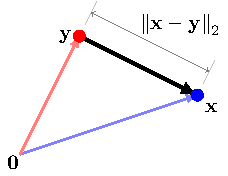
\includegraphics[width=0.95\linewidth]{figure/chapter01/dist-demo.pdf}
        \caption{Distance between two vectors $\mf{x}$ and $\mf{y}$ in $\mb{R}^2$. This figures depicts the 2-norm, but any $p$-norm or valid norm function could be used to quantify the distance between two vectors or points.}
        % \caption{adsgads}
        \label{fig:dist1}
    \end{subfigure}
    \hspace{0.05\textwidth}
    \begin{subfigure}[b]{0.4\textwidth}
        \centering
        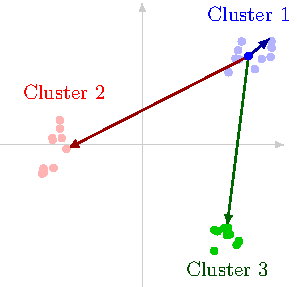
\includegraphics[width=0.85\linewidth]{figure/chapter01/cluster-dist.pdf}
        \caption{Distance between two vectors $\mf{x}$ and $\mf{y}$ in $\mb{R}^2$. This figures depicts the 2-norm, but any $p$-norm or valid norm function could be used to quantify the distance between two vectors or points. Distance between two vectors $\mf{x}$ and $\mf{y}$ in $\mb{R}^2$. This figures depicts the 2-norm, but any $p$-norm or valid norm function could be used to quantify the distance between two vectors or points.}
        \label{fig:dist2}
    \end{subfigure}
    \caption{}
\end{figure}

The similarity between two vectors is measured by the \textit{distance} between the two vectors. The distance between two vectors $\mf{x}, \mf{y} \in \mb{R}^n$ is a function that maps the two vectors to a non-negative real number, and satisfies the following properties:
We looked at the magnitude or size of a vector in the previous section. But vectors also have directions associated with them. If we have two vectors $\mf{x}, \mf{y} \in \mb{R}^n$, then we can ask if these two vectors pointing in similar directions? If the vectors are pointing in the same direction, then they are said to be \textit{collinear}.
% \section{Number theory}
% Figure example
% \begin{figure}[!ht]
%     \centering
%     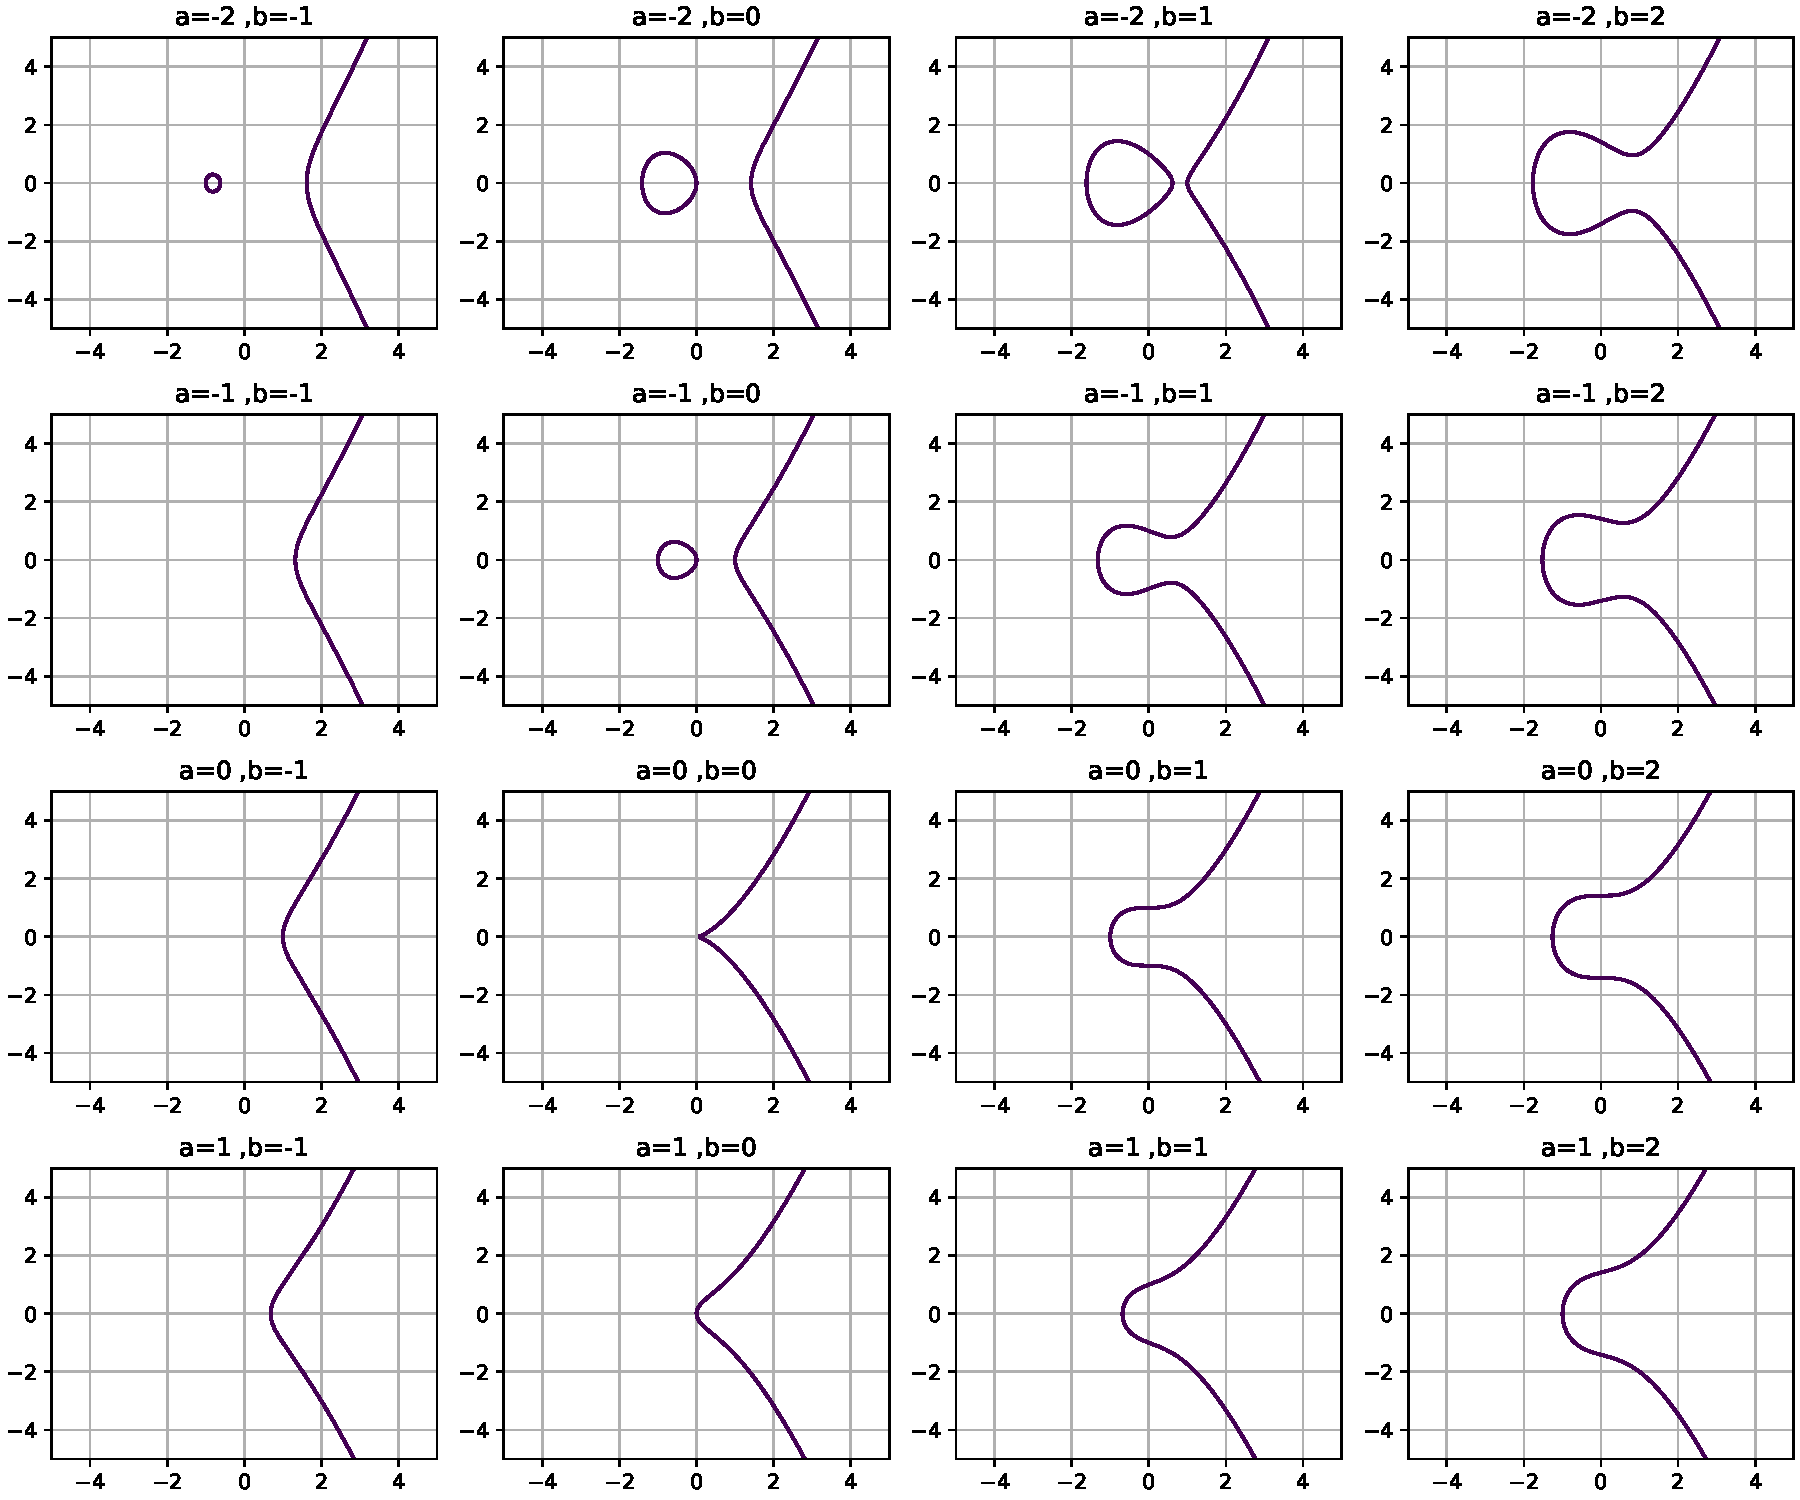
\includegraphics[width=1\linewidth]{./figure/elliptic_curves.pdf}
%     \caption{Elliptic curves \cite{childsUniversalComputationQuantum2009} }
% \end{figure}


% \section{Algorithm}
% % \begin{center}
% % \begin{minipage}{.9\linewidth}
% % algorithm2e
% % https://www.overleaf.com/learn/latex/Algorithms#The_algorithm2e_package
% \begin{algorithm}[H]
%     \SetKwInOut{Input}{input}
%     \SetKwInOut{Output}{output}
%     \Input{Integer $N$ and parameter $1^t$}
%     \Output{A decision as to whether $N$ is prime or composite}
%     \BlankLine
%     \For{ $i = 1,2, \ldots, t$} {
%         $a\leftarrow \qty{1,\dots,N_1}$\;
%         \If{$a^{N-1} \neq 1 \mod{N}$}
%     {\Return "composite"}
%     }
%     \Return "prime"
%     \caption{Primality testing - first attempt}
%     \label{alg:miller_rabin}
% \end{algorithm}
% % \end{minipage}
% % \end{center}